\documentclass[12pt,fleqn]{article}\usepackage{../common}
\begin{document}
Gaussian Karisimlari ile Deri Rengi Saptamak

Bir projemizde dijital resimlerdeki deri rengi iceren kisimlari cikartmamiz
gerekiyordu; cunku fotografin diger renkleri ile ilgileniyorduk (resimdeki
kisinin uzerindeki kiyafetin renkleri) ve bu sebeple deri renklerini ve o
bolgeleri resimde saptamak gerekti. Bizim de onceden aklimizda kalan bir
tembih vardi, Columbia Universitesi'nde yapay ogrenim dersi veren Tony
Jebara derste paylasmisti bir kere (bu tur gayri resmi, lakirdi seviyesinde
tiyolar bazen cok faydali olur), deri rengi bulmak icin bir projesinde tum
deri renklerini R,G,B olarak grafige basmislar, ve beyaz olsun, zenci
olsun, ve sonuc grafikte deri renklerinin cok ince bir bolgede yanyana
durdugunu gormusler. Ilginc degil mi?

Buradan su sonuc cikiyor ki diger renklerin arasinda deri renklerine
odaklanan, onlari ``taniyan'' bir yapay ogrenim algoritmasinin oldukca
sansi vardir. Ama ondan once veriye bakip grafiksel olarak ne oldugunu
gorelim. 

\begin{minted}[fontsize=\footnotesize]{python}
import pandas as pd, zipfile
with zipfile.ZipFile('skin.zip', 'r') as z:
    d =  pd.read_csv(z.open('skin.csv'),sep=',')
print d[:3]
\end{minted}

\begin{verbatim}
   Unnamed: 0   rgbhex   skin         r         g         b         h  \
0           0  #200e08  False  0.125490  0.054902  0.031373  0.041667   
1           1  #6d6565  False  0.427451  0.396078  0.396078  0.000000   
2           2  #1f2c4d  False  0.121569  0.172549  0.301961  0.619565   

          s         v  
0  0.750000  0.125490  
1  0.073394  0.427451  
2  0.597403  0.301961  
\end{verbatim}

Burada onemli olan R,G,B ve H,S,V kolonlari. Bu iki grup degisik renk
kodlama yontemini temsil ediyorlar. Grafikleyelim,

\begin{minted}[fontsize=\footnotesize]{python}
nd = d[d['skin'] == False]
sd = d[d['skin'] == True]
plt.plot(nd['r'],nd['g'],'.')
plt.hold(True)
plt.plot(sd['r'],sd['g'],'rx')
plt.savefig('stat_gmm_01.png')
\end{minted}


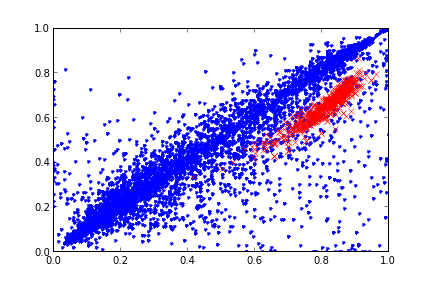
\includegraphics[height=6cm]{stat_gmm_01.png}

Ya da H,S uzerinden

\begin{minted}[fontsize=\footnotesize]{python}
nd = d[d['skin'] == False]
sd = d[d['skin'] == True]
plt.plot(nd['h'],nd['s'],'.')
plt.hold(True)
plt.plot(sd['h'],sd['s'],'rx')
plt.savefig('stat_gmm_02.png')
\end{minted}

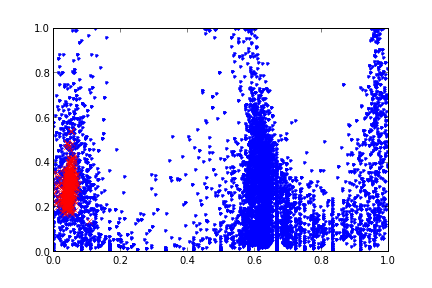
\includegraphics[height=6cm]{stat_gmm_02.png}

Demek ki Jebara hakliymis. Veriye bakinca bir kabaca / sezgisel (intuitive)
bazi cikarimlar yapmak mumkun. Mesela her iki grafikte de deri renklerini
belirten bolgenin grafigi sanki 3 boyutlu bir Gaussian'in ustten gorunen /
kontur (contour) hali. Bunu bilmek bir avantaj, bu avantaji kullanmak
lazim. Eger modelimiz gercek dunya verisine ne kadar yakinsa, yapay ogrenim
sansi o kadar fazlalasacaktir. Eger o bolgeye bir Gaussian uydurursak (fit)
tanima sansimiz artacaktir. 

O zaman deri rengi tanima su sekilde yapilabilir. Scikit Learn
kutuphanesinin Gaussian Karisimlari (GMM) iceren cok guzel bir paketi var,
bunu kullanabiliriz. Tek problem bu karisimlar olasilik fonksiyonunu
ogreniyorlar, siniflama (classification) yapmiyorlar. Onemli degil, soyle
bir ek kod ile bunu halledebiliriz; iki tane GMM yaratiriz, bir tanesi deri
renk bolgeleri icin, digeri diger bolgeler icin. Egitim sirasinda her iki
GMM'i kendi bolgeleri uzerinde egitiriz. Sonra, test zamaninda, her yeni
(bilinmeyen) veri noktasini her iki GMM'e veririz, hangisinden daha yuksek
olasilik degeri geliyorsa, etiket degeri olarak o GMM'in degerini aliriz. 

GMM'leri, ve onlarin icindeki Gaussian'larin kovaryanslarini kullanmak
faydali, kovaryans bildigimiz gibi bir Gaussian'in hangi yonde daha fazla
agirliginin olacagini belirler, eger kovaryans hesabi yapilmazsa, yani
kovaryans matrisinin sadece caprazinda degerler varsa, mesela uc boyutta
Gaussian'in konturu bir cember olarak gozukur [1, sf 90]. Tabii her yonde
ayni agirlikta olan bir Gaussian her turlu veriyi temsil edemez, en esnegi
(ki grafige bakinca bu gerekliligi goruyoruz) tam kovaryans
kullanmaktir. Scikit Learn ile bu secim GMM icin \verb!full! ile yapilir,
sadece caprazi kullan anlamina gelen \verb!diag! da olabilirdi.

\begin{minted}[fontsize=\footnotesize]{python}
import zipfile
from sklearn.cross_validation import train_test_split
from sklearn.metrics import roc_curve, auc
from sklearn.metrics import roc_auc_score
from sklearn.mixture import GMM
import pandas as pd

class GMMClassifier():
   def __init__(self,k,var):
       self.clfs = [GMM(n_components=k,
                    covariance_type=var,thresh=0.1, 
                    min_covar=0.0001,n_iter=100) for i in range(2)]

   def fit(self,X,y):
       self.clfs[0].fit(X[y==0])
       self.clfs[1].fit(X[y==1])

   def predict(self,X):
       res0 = self.clfs[0].score(X)
       res1 = self.clfs[1].score(X)
       res = (res1 > res0)
       return res.astype(float)

if __name__ == "__main__": 
 
   with zipfile.ZipFile('skin.zip', 'r') as z:
      df =  pd.read_csv(z.open('skin.csv'),sep=',')
   y = (df['skin'] == True).astype(float)
   X = df[['h','s','v','r','g']]
   
   res = []   
   for i in range(5):
      clf = GMMClassifier(k=10,var='full')
      x_train, x_test, y_train, y_test = train_test_split(X, y, test_size=2000)
      clf.fit(x_train,y_train)
      preds = clf.predict(x_test)

      fpr, tpr, thresholds = roc_curve(y_test, preds)
      roc_auc = auc(fpr, tpr)
      res.append(roc_auc)

   print 'deneyler', res
   print 'nihai ortalama', np.array(res).mean()
\end{minted}

\begin{verbatim}
deneyler [0.99075081610446136, 0.98417442945172173, 0.98641291695170819,
          0.98779826464208242, 0.99239130434782608] 
nihai ortalama 0.9883055463
\end{verbatim}

Basari orani yuzde 98.8! Bu problem uzerinde pek cok diger yontem denedik,
mesela KNN siniflayici, Lojistik Regresyon, vs. gibi, bu yontem tum
digerlerini gecti. 

Ilginc bir yan bir soru, ``hangi kolonlarin kullanilacagi''. Bu baglamda
projede arkadaslardan ``ama HSV degerleri RGB degerlerinden
turetilebiliyor, ya birini ya otekini kullanmak yeterli olmaz mi?'' yorumu
yapanlar oldu. Evet, bu verinin digerinden ``turetilmis'' oldugu dogru, ve
beklenir ki ideal bir dunyada mukemmel bir yapay ogrenim algoritmasinin bu
tur bir yardima ihtiyaci olmaz, algoritma o kadar iyidir ki ona sanki ayni
veriyi tekrar vermis gibi oluruz, en iyi ihtimalle ek kulfet
yaratiriz. Fakat pratikte bu ek veri algoritmaya ek bazi sinyaller
verebilir. Mesela eger musterilerin kilosu uzerinden bir ogrenim yapiyor
olsaydik, 80 kilodan daha az ya da daha fazla olmayi (problem alanina gore)
ayri bir kolon olarak kodlamak avantaj getirebilirdi. Tabii ki kilo verisi
numerik deger olarak aziyla fazlasiyla oradadir, fakat onem verdigimiz
noktalari turetilmis veri olarak ogrenim algoritmasina vermenin zarari
yoktur. Ustteki ornekte GB degerlerinin HSV ile beraber kullanilmasinin
basari sansini biraz daha arttirdigini gorebiliriz.

Kaynaklar

[1] Alpaydin, E., {\em Introduction to Machine Learning}

[2] Jebara, T., {\em Columbia Machine Learning Course}


\end{document}
